\documentclass[letter]{article}
\usepackage[cm]{fullpage}
\usepackage[table]{xcolor}
\usepackage{listings}
\usepackage{graphicx}
\usepackage{hyperref}
%package below is for adding images in exact place in code
\usepackage{float}
\usepackage[toc,page]{appendix}

 
\setlength{\arrayrulewidth}{1mm}
\setlength{\tabcolsep}{18pt}
\renewcommand{\arraystretch}{2.5}

\graphicspath{ {images/} }

%background color for source code snippets and links 
\definecolor{mygray}{gray}{0.95}

%for changing color in links
\hypersetup{
    colorlinks,
    linkcolor={black},
    citecolor={blue!50!black},
    urlcolor={blue!80!black}
}

%source code with highliting
\lstset{basicstyle=\fontsize{9}{10}\ttfamily,
	backgroundcolor=\color{mygray},
  	%commentstyle=\color{blue},
  	%keywordstyle=\color{blue}
	language=bash,
	xleftmargin=\parindent,
	extendedchars=true, 
	showspaces=false,
	showstringspaces=false,
}

%for an src directory of bash scripts
\newcommand*\lstinputpath[1]{\lstset{inputpath=#1}}
\lstinputpath{src}

%prints out helpful info with layout uncommented below
%\usepackage{layout}

\title{Performance Analysis on Intel XL710 using DPDK i40e Poll Mode Driver \\ Tests on ppc64le using DPDK v17.11}
\author{Mick Tarsel \\  LTC Networking Team \\}  

\begin{document}
%\layout

\maketitle

\newpage
\tableofcontents
\newpage

\section{Machine Information}
%to many 1 line explanations that should not be indented.
{\setlength{\parindent}{0cm}

Using 2 Power 8 machines each with 2 XL710 i40e 40Gbs NICs.

Both machines have the following configurations:
\begin{itemize}
\item smt=off
\item NUMA=off
\item rx buffer 1024 (except for I/O with 2 ports)
\item tx buffer 512
\item hugepage size 16mb
\item number of hugepages 1024
\end{itemize}

The machine running pktgen, sending traffic, is Ubuntu 17.04 with kernel 4.10.0-35-generic.
\begin{lstlisting}[escapechar=!]
$ cat /proc/cmdline
hugepages=1024 isolcpus=40-43,48-51,56-59
\end{lstlisting}
 
DPDK is running on RHEL 7.4 with kernel 3.10.0-693.1.1.el7.ppc64le
\begin{lstlisting}[escapechar=!]
$ cat /proc/cmdline
hugepages=1024 isolcpus=40-43,48-51,56-59 numa=off
\end{lstlisting}
Any refernce to another section will be a clickable link to that section.

%%%%%%%%%%%%%%%%%%%%%%%%%%%%%%%%%%%%%%%%%%%%%%%%%%%%%
%%%  RX only bandwidth using testpmd
%%%%%%%%%%%%%%%%%%%%%%%%%%%%%%%%%%%%%%%%%%%%%%%%%%%%%

\section{RX Only Bandwidth using testpmd}
%to many 1 line explanations that should not be indented.
{\setlength{\parindent}{0cm}

\begin{figure}[H]
%\caption{some caption}
\hbox{\vspace{0.5cm}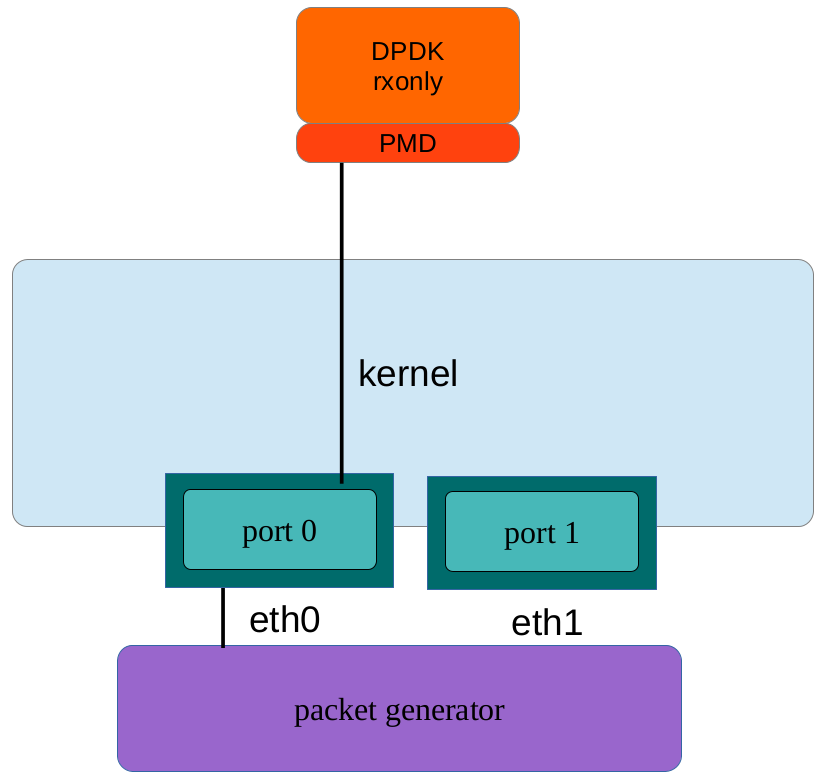
\includegraphics[scale=0.4]{rx-only} }
\end{figure}

\subsection{Results}
\large
\begin{center}
\begin{tabular}{ |c|c|c|c|c|c| }
\hline
\multicolumn{6}{|c|}{RX Only Results} \\
 \hline
 pkt size (bytes) & 64 & 128 & 256 & 512 & 1024\\ 
\hline
 pktgen Mpps & 59.96 & 34.318 & 18.15 & 9.42 & 4.79\\ 
 rx only Mpps & 24.86 & 24.88 & 24.27 & 12.59 & 6.41\\ 
\hline
\rowcolor{yellow}
\% rate & 41.46 & 72.5 & ? & ? & ?\\
 \hline
\end{tabular}
\end{center}

\subsection{pktgen Machine (126)}

% ./pktgen -l 0-3,8-11,16-19,24-27,32-35,40-43,48-51,56-59,64-67,72-75 --socket-mem=4096,4096 -- -T -P -m "[8:40-43/48-51].0"
\begin{lstlisting}
pktgen -l 0-3,8-11,16-19,24-27,32-35,40-43,48-51,56-59,64-67,72-75 --socket-mem=4096,4096 
	-- -T -P -m "[8:40-43/48-51].0"
\end{lstlisting}

\subsection{testpmd (124)}

% Q=8; testpmd -l 0,8,16,24,32,40,48,56,64,72 -m 4096 -w 0002:01:00.0 -- --txd=512 --rxd=1024 --mbcache=512 --rxq=$Q--txq=$Q --nb-cores=$Q -i -a --rss-ip --forward-mode=rxonly  --port-topology=chained
\begin{lstlisting}[escapechar=!]
Q=8; testpmd -l 0,8,16,24,32,40,48,56,64,72 -m 4096 -w 0002:01:00.0 
-- --txd=512 --rxd=1024 --mbcache=512 --rxq=$Q--txq=$Q --nb-cores=$Q -i -a 
	--rss-ip --forward-mode=rxonly  --port-topology=chained
\end{lstlisting}

\subsection{Starting Test}

\begin{lstlisting}[escapechar=!]
Pktgen:/> start 0
\end{lstlisting}

\begin{lstlisting}
testpmd> show port stats all

  ######################## NIC statistics for port 0  ########################
  RX-packets: 16519665   RX-missed: 0   RX-bytes:  3885350400
  RX-errors: 0
  RX-nombuf:  0         
  TX-packets: 16         TX-errors: 0          TX-bytes:  0

  Throughput (since last show)
  Rx-pps:     24898418
  Tx-pps:            0
  ############################################################################
testpmd> 
\end{lstlisting}




%%%%%%%%%%%%%%%%%%%%%%%%%%%%%%%%%%%%%%%%%%%%%%%%%%%%%
%%% I/O forward across 2 ports
%%%%%%%%%%%%%%%%%%%%%%%%%%%%%%%%%%%%%%%%%%%%%%%%%%%%%
\section{I/O forward bandwidth using testpmd across ports}

\begin{figure}[H]
%\caption{Path of ICMP packet from \texttt{namespace1} through \texttt{br-1} to \texttt{namespace2}}
\hbox{\hspace{-0.5cm} 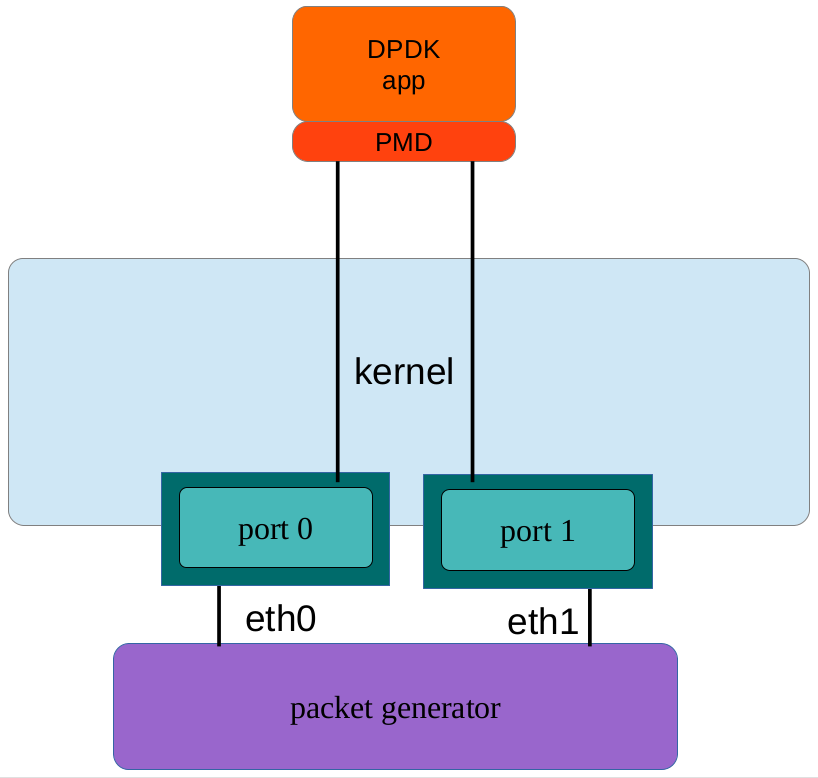
\includegraphics[scale=0.6]{i-o-2-ports} }
\end{figure}

\subsection{Results}
\large
\begin{center}
\begin{tabular}{ |c|c|c|c|c|c| }
\hline
\multicolumn{6}{|c|}{RX Only Results} \\
 \hline
 pkt size (bytes) & 64 & 128 & 256 & 512 & 1024\\ 
\hline
 pktgen Mpps & 59.96 & 34.06 & 18.15 & 9.42 & 4.79\\ 
 I/O Mpps & 20.12 & 20.12 & 20.12 & 12.59 & 6.41\\ 
\hline
\rowcolor{yellow}
\% rate & 34.07 & 59.07 & ? & ? & ?\\
 \hline
\end{tabular}
\end{center}

\subsection{pktgen Machine (126)}

% ./pktgen -l 0-3,8-11,16-19,24-27,32-35,40-43,48-51,56-59,64-67,72-75 --socket-mem=4096,4096 -- -T -P -m "[8:40-43/48-51].0,[56-59/64-67:72].1"
\begin{lstlisting}
pktgen -l 0-3,8-11,16-19,24-27,32-35,40-43,48-51,56-59,64-67,72-75 --socket-mem=4096,4096 
	-- -T -P -m "[8:40-43/48-51].0,[56-59/64-67:72].1"
\end{lstlisting}

\subsection{testpmd (124)}

% testpmd -l 0,8,16,24,32,40,48,56,64,72 -m 4096 -w 0002:01:00.0 -w 0002:01:00.1 -- --txd=512 --rxd=1024 --mbcache=512 --rxq=$Q --txq=$Q --nb-cores=$Q -i -a --rss-ip --forward-mode=io
\begin{lstlisting}[escapechar=!]
Q=8; testpmd -l 0,8,16,24,32,40,48,56,64,72 -m 4096 -w 0002:01:00.0 -w 0002:01:00.1 -- --txd=512
--rxd=1024 --mbcache=512 --rxq=$Q --txq=$Q --nb-cores=$Q -i -a --rss-ip --forward-mode=io
\end{lstlisting}

\subsection{Starting Test}

\begin{lstlisting}[escapechar=!]
Pktgen:/> enable 0 range
-- Pktgen 
Pktgen:/> start 0
\end{lstlisting}

\begin{lstlisting}
Port 0: LSC event
Port 1: LSC event
testpmd> show port stats all
testpmd> show port stats all

  ######################## NIC statistics for port 0  ########################
  RX-packets: 15107923   RX-missed: 62402292   RX-bytes:  4650612480
  RX-errors: 0
  RX-nombuf:  0         
  TX-packets: 30         TX-errors: 0          TX-bytes:  1440

  Throughput (since last show)
  Rx-pps:     20292924
  Tx-pps:            5
  ############################################################################

  ######################## NIC statistics for port 1  ########################
  RX-packets: 30         RX-missed: 0          RX-bytes:  1440
  RX-errors: 0
  RX-nombuf:  0         
  TX-packets: 15108497   TX-errors: 0          TX-bytes:  906509264

  Throughput (since last show)
  Rx-pps:            5
  Tx-pps:     20292567
  ############################################################################
testpmd> 

\end{lstlisting}


%%%%%%%%%%%%%%%%%%%%%%%%%%%%%%%%%%%%%%%%%%%%%%%%%%%%%
%%% I/O forward across 1 port
%%%%%%%%%%%%%%%%%%%%%%%%%%%%%%%%%%%%%%%%%%%%%%%%%%%%%
\section{I/O forward bandwidth using testpmd within same port}
%to many 1 line explanations that should not be indented.
{\setlength{\parindent}{0cm}

\begin{figure}[H]
%\caption{Path of ICMP packet from \texttt{namespace1} through \texttt{br-1} to \texttt{namespace2}}
\hbox{\hspace{-0.5cm} 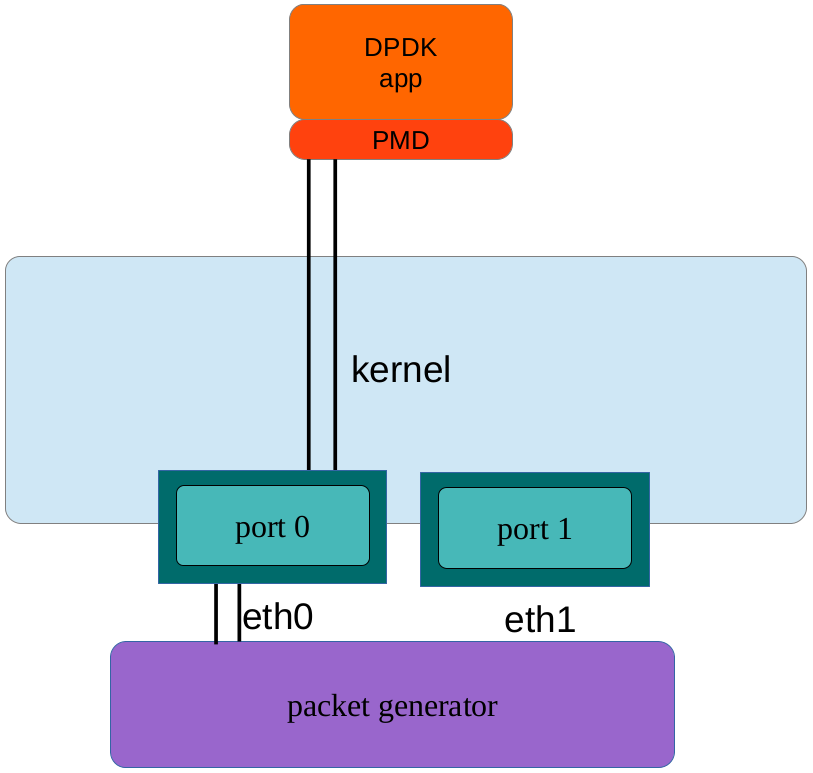
\includegraphics[scale=0.6]{i-o-1-port} }
\end{figure}

\subsection{Results}
\large
\begin{center}
\begin{tabular}{ |c|c|c|c|c|c| }
\hline
\multicolumn{6}{|c|}{RX Only Results} \\
 \hline
 pkt size (bytes) & 64 & 128 & 256 & 512 & 1024\\ 
\hline
 pktgen Mpps & 59.96 & 34.06 & 18.15 & 9.42 & 4.79\\ 
 I/O Mpps & 23.01 & 23 & 23 & 12.59 & 6.41\\ 
\hline
\rowcolor{yellow}
\% rate & 38.38 & 67.53 & ? & ? & ?\\
 \hline
\end{tabular}
\end{center}

\subsection{pktgen Machine (126)}

% ./pktgen -l 0-3,8-11,16-19,24-27,32-35,40-43,48-51,56-59,64-67,72-75 --socket-mem=4096,4096 -- -T -P -m "[8-11/16-19:40-43/48-51].0"
\begin{lstlisting}
pktgen -l 0-3,8-11,16-19,24-27,32-35,40-43,48-51,56-59,64-67,72-75 
	--socket-mem=4096,4096 -- -T -P -m "[8-11/16-19:40-43/48-51].0"
\end{lstlisting}

\subsection{testpmd (124)}

% testpmd -l 0,8,16,24,32,40,48,56,64,72 -m 4096 -w 0002:01:00.0 -- --txd=512 --rxd=1024 --mbcache=512 --rxq=$Q --txq=$Q --nb-cores=$Q -i -a --rss-ip --forward-mode=io 
\begin{lstlisting}[escapechar=!]
Q=8; testpmd -l 0,8,16,24,32,40,48,56,64,72 -m 4096 -w 0002:01:00.0 -- --txd=512 
--rxd=1024 --mbcache=512 --rxq=$Q --txq=$Q --nb-cores=$Q -i -a --rss-ip --forward-mode=io
\end{lstlisting}

\subsection{Starting Test}

\begin{lstlisting}[escapechar=!]
Pktgen:/> enable 0 range
-- Pktgen 
Pktgen:/> start 0
\end{lstlisting}

\begin{lstlisting}
Port 0: LSC event
testpmd> show port stats all

  ######################## NIC statistics for port 0  ########################
  RX-packets: 27704184   RX-missed: 42793993   RX-bytes:  4229888660
  RX-errors: 0
  RX-nombuf:  0         
  TX-packets: 27704037   TX-errors: 0          TX-bytes:  1662241920

  Throughput (since last show)
  Rx-pps:     23247541
  Tx-pps:     23247573
  ############################################################################
testpmd>
\end{lstlisting}

%%%%%%%%%%%%%%%%%%%%%%%%%%%%%%%%%%%%%%%%%%%%%%%%%%%%%
%%% PVP
%%%%%%%%%%%%%%%%%%%%%%%%%%%%%%%%%%%%%%%%%%%%%%%%%%%%%

%Q=8; testpmd -l 0,8,16,24,32,40,48,56,64,72 -m 2048 -w 0002:01:00.0 -w 0002:01:00.1 --vdev 'net_vhost0,iface=/var/run/openvswitch/vhost-vm1' --vdev 'net_vhost1,iface=/var/run/openvswitch/vhost-vm2' -- --txd=512 --rxd=1024 --mbcache=512 --rxq=$Q --txq=$Q --nb-cores=$Q -i -a --rss-ip --forward-mode=io

% ./pktgen -l 0-3,8-11,16-19,24-27,32-35,40-43,48-51,56-59,64-67,72-75 --socket-mem=4096,4096 -- -T -P -m "[8:40-43/48-51].0,[56-59/64-67:72].1"

}%for no indents on one-liners

\end{document}

